\documentclass[dvisvgm,border=2pt]{standalone}
% Shared by every figure. Two colours only: black becomes the text colour of
% whatever theme the app is in, and `accent` becomes the brand — see
% scripts/build-figures.mjs. Everything else is done with opacity.
\usepackage{amsmath}
\usepackage{amssymb}
\usepackage{tikz}
\usepackage{pgfplots}
\pgfplotsset{compat=1.18}
\usetikzlibrary{arrows.meta,positioning,calc,backgrounds,fit,patterns.meta}
\definecolor{accent}{RGB}{255,0,255}
\pgfplotsset{
  every axis/.append style={
    axis lines=left,
    axis line style={draw opacity=0.35},
    tick style={draw opacity=0.35},
    tick label style={font=\scriptsize,opacity=0.7},
    label style={font=\scriptsize,opacity=0.7},
    legend style={draw=none,fill=none,font=\scriptsize},
    every axis plot/.append style={line width=0.7pt},
  },
}
\tikzset{
  every picture/.style={font=\scriptsize},
  faint/.style={opacity=0.3},
  quiet/.style={opacity=0.55},
  box/.style={draw,opacity=0.35,rounded corners=2pt,inner sep=4pt},
  hot/.style={accent},
}

\begin{document}
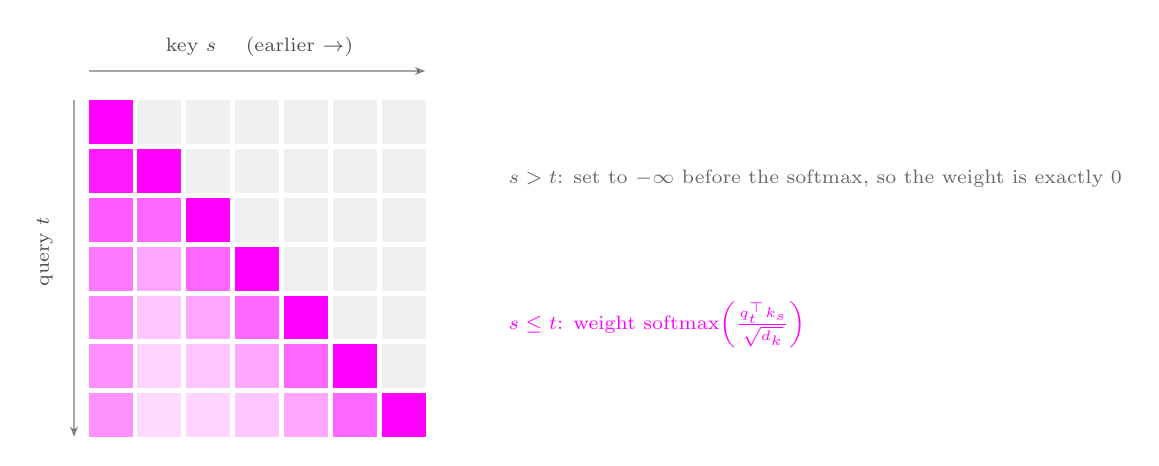
\begin{tikzpicture}[scale=0.62]
  \foreach \i in {0,...,6}{
    \foreach \j in {0,...,6}{
      \pgfmathsetmacro{\w}{\j<=\i ? 0.12+exp(-0.75*(\i-\j))+(\j==0 ? 0.3 : 0) : 0}
      \ifnum\j>\i
        \fill[opacity=0.06] (\j,-\i) rectangle ++(0.9,-0.9);
      \else
        \fill[accent,opacity=\w] (\j,-\i) rectangle ++(0.9,-0.9);
      \fi
    }
  }
  \node[opacity=0.7,rotate=90] at (-0.9,-3.1) {query $t$};
  \node[opacity=0.7] at (3.5,1.1) {key $s$ \quad (earlier $\rightarrow$)};
  \draw[opacity=0.35,-{Stealth[length=4pt]}] (0,0.6) -- (6.9,0.6);
  \draw[opacity=0.35,-{Stealth[length=4pt]}] (-0.3,0) -- (-0.3,-6.9);
  \node[opacity=0.6,align=left,anchor=west] at (8.4,-1.6)
    {$s>t$: set to $-\infty$\ before the softmax,\ so the weight is exactly $0$};
  \node[accent,align=left,anchor=west] at (8.4,-4.6)
    {$s\le t$: weight\ $\mathrm{softmax}\!\left(\frac{q_t^{\top}k_s}{\sqrt{d_k}}\right)$};
\end{tikzpicture}
\end{document}
